%
% Spark reference architectures
% Copyright (C) 2016 Martin Zapletal
%
% This program is free software: you can redistribute it and/or modify
% it under the terms of the GNU General Public License as published by
% the Free Software Foundation, either version 3 of the License, or
% (at your option) any later version.
%
% This program is distributed in the hope that it will be useful,
% but WITHOUT ANY WARRANTY; without even the implied warranty of
% MERCHANTABILITY or FITNESS FOR A PARTICULAR PURPOSE.  See the
% GNU General Public License for more details.
%
% You should have received a copy of the GNU General Public License
% along with this program.  If not, see <http://www.gnu.org/licenses/>.
%

\documentclass[a4paper, 10 pt, conference]{IEEEtran}

\usepackage{graphicx}
\usepackage{interval}
\usepackage{listings}
\usepackage{hyperref}
\usepackage{siunitx}
\usepackage{amsmath}

\sisetup{load-configurations = abbreviations, binary-units = true}
\intervalconfig {
soft open fences ,
separator symbol =; ,
}

\title{Spark Reference Architecture \\ Financial transactions streaming}

\author{Martin Zapletal%$^{1}$% <-this % stops a space
%\thanks{Supported by Cake Solutions Limited}% <-this % stops a space
%\thanks{$^{1}$Martin Zapletal is the CTO at Cake Solutions Inc., 195 Plymout Street, 11201, New York {\tt\small martinz at cakesolutions.net}}%
}


\begin{document}

\maketitle
\thispagestyle{empty}
\pagestyle{empty}

%%%%%%%%%%%%%%%%%%%%%%%%%%%%%%%%%%%%%%%%%%%%%%%%%%%%%%%%%%%%%%%%%%%%%%%%%%%%%%%%
\begin{abstract}
This document describes distributed, large data volume stream processing architecture that was used in a real life production financial transaction processing system. The system receives input data from files at defined times and at the same time continuously ingests data from a streaming integration point, processes and transforms the data as a stream, validates them against known records and finally stores the results.

The document describes architecture, technology choices, explanation of system requirements such as data consistency, integrity, performance, fault tolerance or availability and how the selected technologies and their interoperability fulfil the requirements, focusing on Apache Spark. Cluster and resource management required to fulfil some of the requirements as well as to improve cluster utilisation and achieve financial savings are also thoroughly discussed. Finally scenarios where selected technologies and architecture can not be applied due to specific limitations are discussed.
\end{abstract}


%%%%%%%%%%%%%%%%%%%%%%%%%%%%%%%%%%%%%%%%%%%%%%%%%%%%%%%%%%%%%%%%%%%%%%%%%%%%%%%%
\section{Introduction}

\subsection{Spark components}
This reference architecture uses Spark Core, Spark Streaming and Spark SQL.

\subsection{Non Spark components}

Apart from Apache Spark this reference architecture makes use of Cassandra, Kafka, Filesystem, S3 and Elasticsearch.

\subsection{Resource manager}
For automated deployment, infrastructure and operations and resource management Mesosphere Datacenter Operating System (CS/OS) is used.

\section{Reference implementation}

The application receives multiple types of inputs. One are files from other financial institution uploaded at defined times to an integration point and containing a set of transactions. The other one is integration with other systems through Apache Kafka. The records are processed, validated against known data stored in Cassandra database, transformed and finally stored in Cassandra and relevant information sent to integration points with other internal systems. In addition generation of report sand analytics from the stored result data is required. The application has strict requirements for uptime, availability, consistency, data integrity, scalability and cost optimisation while ideally using OS technologies. For those reasons Mesosphere DSOS was chosen for infrastructure automation, cluster and resource management.

\section{Main components}

The main components in this architecture are data sources (file source and Apache Kafka), stream processing pipeline and database. High level architecture is displayed on figure~\ref{fig:components}. 

\begin{figure}[hb]
	\begin{center}
		\caption{Components}
		\label{fig:components}
		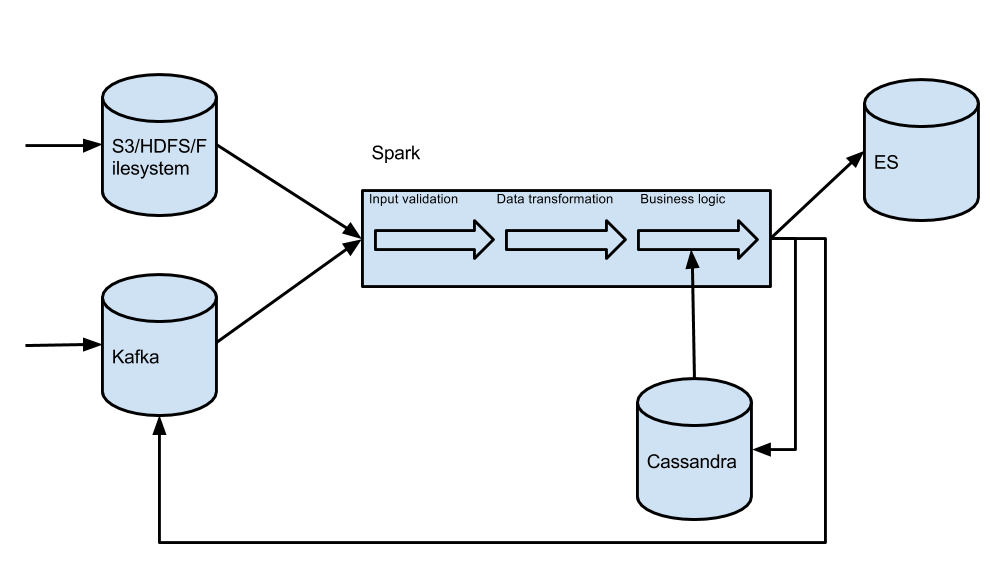
\includegraphics[width=8cm,keepaspectratio]{architecture-diagram.png}
	\end{center}
\end{figure}

\subsection{Data sources}
In this reference architecture two different data sources are used. An input directory is used for historical reasons as an integration point between financial institutions. A file in a known format is uploaded to the directory in defined intervals. Apache Spark file stream source can monitor a directory and process each new file as it is added to the directory. Batch processing capability of Apache Spark was preferred in this case for reasons explained later in section about cluster scheduling and resource management.
Apache Kafka is used for integration with other internal systems. Kafka is a distributed log often used for integration for its scalability, reliability, durability, replayability and other attributes. Spark Streaming provides a Kafka input stream and its direct version as options to stream data from Kafka.

\subsection{Stream processing}
After ingesting data from the sources they need to go through a processing pipeline with guarantees satisfying the requirements. The requirements and guarantees provided by Spark are in detail described in next section.
The stream processing pipeline is used for the following purposes.

\subsubsection{Input cleaning and validation}
The inputs are validated. For example the input may not be in the correct format, expected schema invalid, required fields may be missing, outliers may be checked, input data from different publishers standardised and cleaned or other validation done and data filtered.

\subsubsection{Data transformation}
Before processing the data we may need to transform the data into correct format. That may involve transforming from XML/json/cvs/binary or other data format to business logic representation that is easier and safer to work with, query and analyse.

\subsubsection{Business logic implementation}
After the data are in correct format for processing we can apply the actual business logic rules. It may involve queries, real time analytics, aggregations, training and application of machine learning model or asynchronous communication with other systems. In this particular architecture the input data are validated and enriched using records stored in Cassandra database.

\subsubsection{Data storage}
The processed data are stored in a database solution. Firstly, the business logic records are updated using the previously applied business rules. Secondly, an analytics data store is updated with the new records for advanced analytics and search purposes. 

// TODO: Updates to storage and analytics storage
// TODO: Direct updates vs via the platform

\subsubsection{Result integration}
Enterprise systems are often large distributed application consisting of many services, independent applications and modules. Spark is used to provide updates about the real time processing to the interested services by publishing a stream to Apache Kafka. Kafka is then used as streaming data platform for other systems to subscribe to real time updates with Kafka's strong guarantees.

\section{Streaming data platform}

\begin{figure}[hb]
	\begin{center}
		\caption{Streaming data platform}
		\label{fig:streamingDataPlatform}
		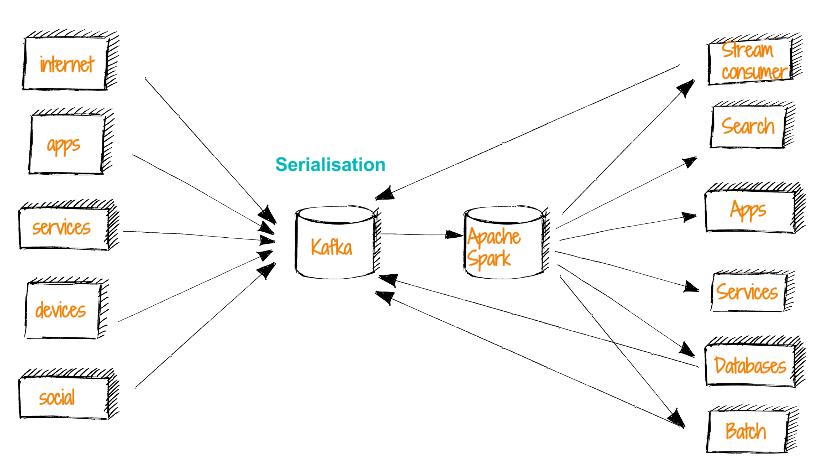
\includegraphics[width=8cm,keepaspectratio]{streaming-data-platform.png}
	\end{center}
\end{figure}

Commonly, ETL and data processing was done in batches and batch processing architectures, supported by Hadoop and similar technologies was common. Due to lack of flexibility and often slow results Lambda Architecture was introduced. It uses batch layer to still deliver correct result and streaming layer to deliver some or partial results quickly.
ETL and batch processes were still often run in intervals capturing a current snapshot of the data to mimic streaming, often due to insufficient access to streaming solutions. The approaches to data processing were questioned with the introduction of Streaming data platform (sometimes called Kappa architecture) in [https://www.oreilly.com/ideas/questioning-the-lambda-architecture] displayed on figure~\ref{fig:streamingDataPlatform}.

This architecture uses a solution that can handle large scale streaming data such as Apache Kafka. Any team, application, system, service, sensors, devices etc. can publish their data into the streaming platform. On the consumer side anyone can subscribe to the streaming data platform and consume the streams they are interested in. They are kept up to date with the latest data using a streaming solution and depend on guarantees a particular streaming solution offers.
The advantages compared to batch processing are obvious. Not only are the same guarantees of batch processing maintained, but the consumers are kept up to date in near real time.
Apache Spark Streaming module fits very well into such architecture with reliable delivery, fault tolerance, throughput, scalability and integration with many other streaming solutions. It is used as a consumer and for transformation, repartitioning of data and preparation for the subscribers to use efficiently as displayed on figure~\ref{fig:streamingDataPlatform}.

\section{Requirements and Spark's guarantees}

\subsection{Data consistency}
The application requires strong consistency guarantees (not in strong serializability database transaction sense sense). The data must always be processed and the result correctly updated. All records from an incoming file or Kafka connector must be processed. 

\subsection{Delivery guarantees}
The application also requires exactly once delivery guarantees. Each element read from either file or Kafka must be delivered exactly once. In distributed environment this is not trivial, because of unbounded delays, lost messages, failed nodes and asynchronous partial failures. In general case durable persistence on both sides of the pipeline is required, because if a message was acknowledged before processing by the receiver, it could result in loss and if it is acknowledged after processing the receiver can receive duplicates (after retry). Exactly once delivery guarantee problem can be reduced to at least once delivery guarantee by using unique identifiers, idempotence or simplified by using probabilistic data structures to filter duplicate data.

Spark provides exactly once delivery guarantee with additional solutions to non replayable sources (replicating the processing pipeline, storing received data immediately into a durable store), parallel recovering from failures optimisations etc.

TODO: COMPLETE http://www.cakesolutions.net/teamblogs/spark-streaming-tricky-parts

\subsection{Fault tolerance}
To fulfil the consistency and delivery requirements fault tolerance is a must. Spark handles node failures, lost data and other common failures in large scale distributed deployments automatically abstracting all that from the application developer.

Fault tolerance guarantees are discussed in more detail in section about cluster management, because Spark's capabilities can be further enhanced by it.

Worker nodes launch and monitors job's executors. When worker fails, all its child process are also gone. Then the worker process is automatically relaunched, processes restarted and tasks reran. When just the Executor process fails, then it is automatically relaunched by the Worker process and any tasks that were in flight are rescheduled. Stream receivers follows the same resiliency characteristics as 
executors.

TODO: COMPLETE (parallel recovery)

\begin{figure}[hb]
	\begin{center}
		\caption{Spark Streaming Failure Impact}
		\label{fig:sparkStreamingFailureImpact}
		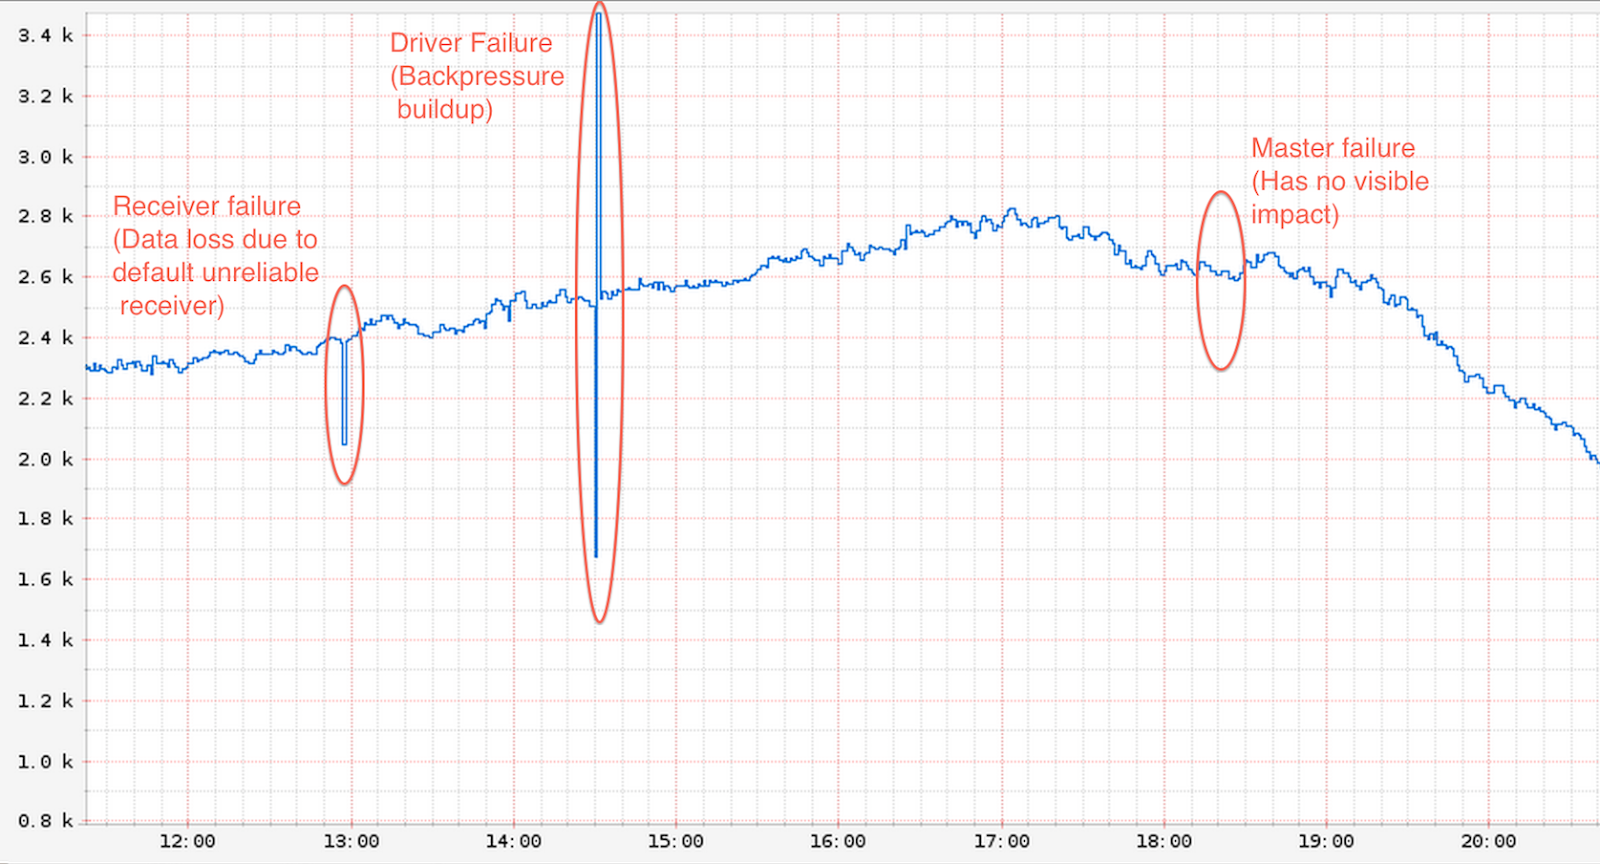
\includegraphics[width=8cm,keepaspectratio]{spark-streaming-failure-impact.png}
	\end{center}
\end{figure}

Failure recovery has impact on the performance ... as displayed on figure~\ref{fig:sparkStreamingFailureImpact}.

Fault tolerance of different spark components is discussed in detail later in section about cluster managers.

\subsection{Order}
Ordering
I processing

TODO: COMPLETE

\subsection{Scalability}
The batch part of the pipeline has strict scalability guarantees. Granularly, on demand submitted batch processes were preferred for their simplicity of deployment, version upgrades, elasticity, ability to assign very different resources to different types of processed files and financial savings. Streaming and a long running repeatedly polling batch process were also considered, but were rejected due to worse granularity, utilisation and flexibility of the solution.

Different inputs are received at different times and have very different profile of core/ram usage and other resource requirements. Keeping all the resources in the cluster available at all times would be very expensive. The ability to scale the size of the cluster up and down elastically is very important. The pattern could look 

\begin{table}[h]
\caption{Processing times requirements}
\label{tbl:processing-times-requirements}
\begin{center}
  \begin{tabular}{ | l | p{3cm} | }
    \hline
    Between 08:00 and 10:00 & run a defined number of ingestion jobs and a defined number of other transaction ingestion jobs.  \\ \hline
    Between 10:00 and 12:00 & execute ingestion jobs ? as many as the current infrastructure will support. \\ \hline
    At 12:00 & execute a transaction reporting extract using all cluster resorces \\ \hline
    When the above has finished & run housekeeping jobs in parallel ? sharing the cluster resources to prepare for next run \\
    \hline
  \end{tabular}
\end{center}
\end{table}

Spark in cooperation with DC/OS provides capabilities to efficiently utilise provisioned resources. Using e.g. a public cloud infrastructure and utilising the pricing strategy it is possible to achieve significant financial savings.
 
 
TODO: COMPLETE https://docs.google.com/document/d/1jdPtcDyRXWheIQ4MLJpXeK4IoxtUrcThou6LmkUaN28/edit
The stream processing pipeline scaling is 

\section{Cluster management and resource scheduler}
Elasticity
Dynamic
Dynamic changes to pipeline

Some of the questions that need to be resolved with regards to resource management are

\begin{itemize}
  \item How to schedule allocation of more resources of the total available for Spark in specific time window during the day? Or react to the number of requests? (fully utilise existing resources in the stack)
  
  \item How to set priorities based on the Spark job type and based on time?
  
  \item How to react to the change in the number of available servers during the day, so it can allocate more resources for Spark when the total available servers increased, and shrink that when they decrease? (Reactively Scale to demand - Both up and Down) 
  
  \item What metrics does it provide for current tasks and finished tasks? (Monitoring of Spark jobs)

  \item Which Spark job approach is more suitable  (Long Running (Streaming) / Job per file / More Granular jobs) 
    
\end{itemize}

Generally we want to utilise available cluster resources as well as possible for Spark jobs and other applications running in the cluster resulting in fault tolerance, performance and also financial savings. 

\begin{figure}[hb]
	\begin{center}
		\caption{Dynamic scaling}
		\label{fig:dynamicScaling}
		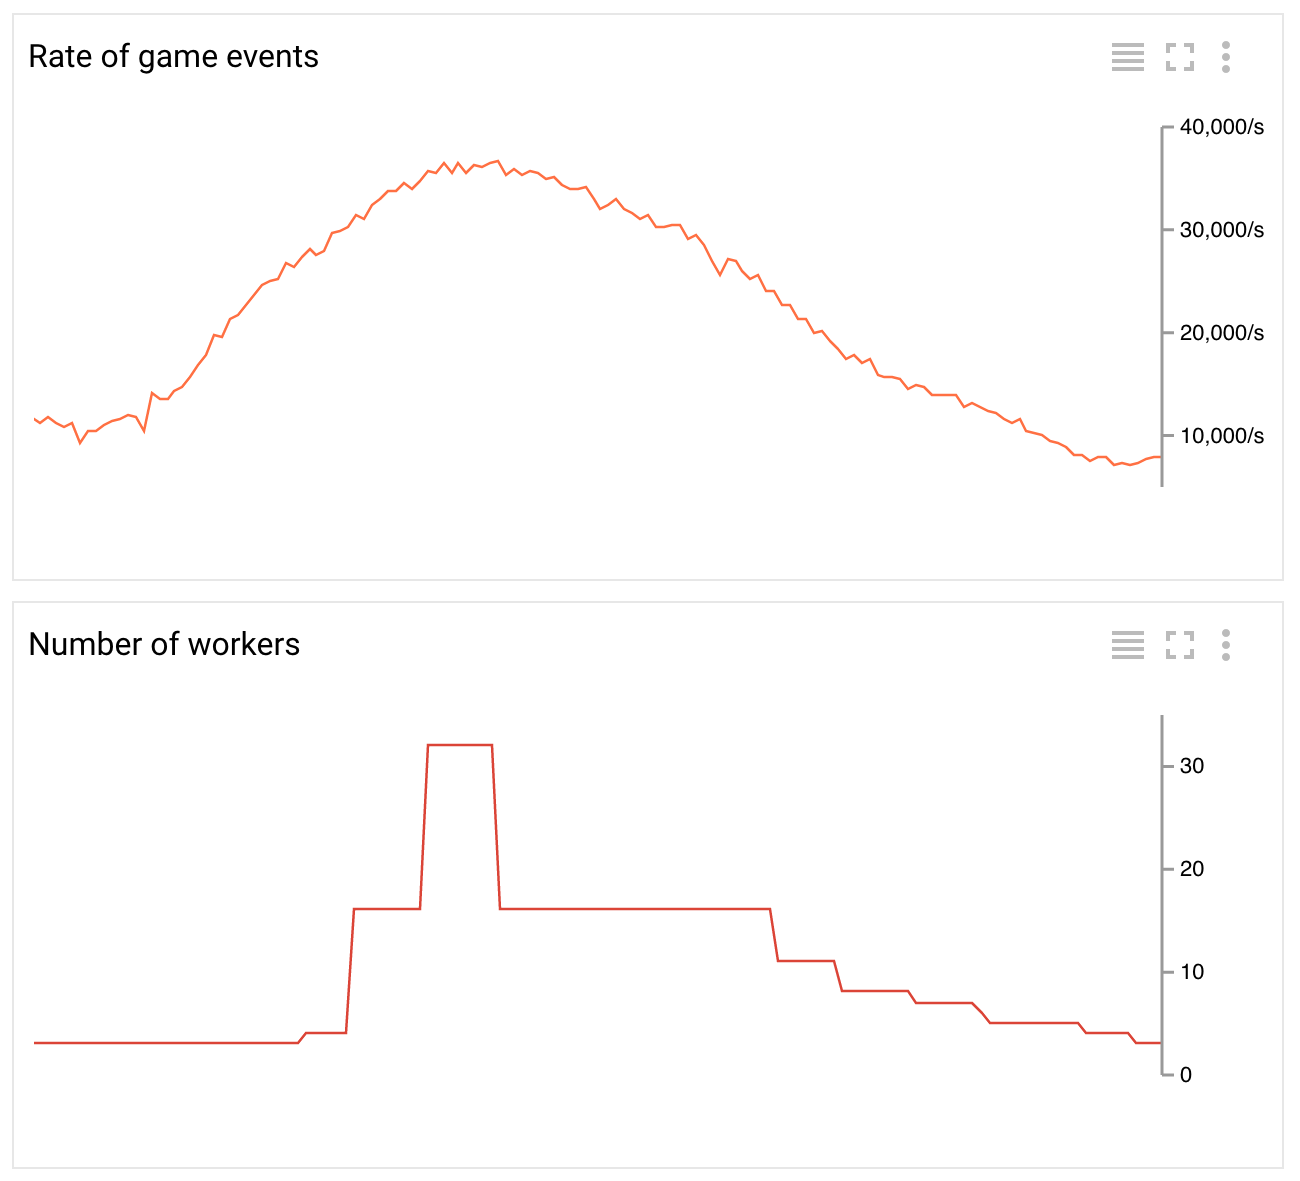
\includegraphics[width=8cm,keepaspectratio]{comparing-s-h-14.png}
	\end{center}
\end{figure}

An example of dynamic scaling based on load in Google Cloud Dataflow is on figure~\ref{fig:dynamicScaling} [https://cloud.google.com/blog/big-data/2016/03/comparing-cloud-dataflow-autoscaling-to-spark-and-hadoop]. Ideally we would want to also keep the number of provisioned (physical) machines to minimum, but never under-provision the cluster to be unable to handle current load. Excessive machines would ideally be returned to provider so they don't have to be paid for. If dynamic cluster sizing is not possible, utilisation still should be maximised between Spark and other applications.

Spark currently can use Standalone mode, YARN or Mesos as a cluster manager. The decision which one to use is very important, because it will determine the capabilities of the cluster and also Spark itself. For implementation of this architecture Mesos/Mesosphere DC/OS was chosen. This section will very briefly discuss capabilities of the other options and then focus on DC/OS and the features that were important for this project.

\subsection{Standalone}
In standalone mode Spark does not rely on any 3rd party cluster manager. Standalone mode provides basic resource scheduling and fault tolerance capabilities. If Spark master crashes, no new application can be created, so it needs a high availability scheme in order to circumvent this. ZooKeeper can be used to provide leader election by launching multiple Spark masters connected to the same ZooKeeper instance. Only one will be elected a leader and the other will remain in standby until the leader is lost. This setup is highly recommended in production scenarios, although it requires a Zookeeper cluster.
Job fault tolerance is managed by Spark itself - if worker nodes crash, Spark automatically reruns the lost part of the computation graph on a different worker node. If the application runs in cluster mode and exits with non-zero code it can be restarted automatically if desired.
Additionally local filesystem can be used to allow applications to recover their state from master crashes.
Spark standalone offers only basic resource management capabilities and scheduling capabilities do not exist at all. By default a FIFO scheduler is used and each job requests and consumes all CPUs available in the cluster. It is not a sufficient solution for multiple user/job scenarios. The only option then is to set up maximum cores for each job using a configuration value. Such solution still does not guarantee efficient utilisation of cluster resources, reactions to changes in load or optimised allocation of resources to each job. The latter can be further improved by empirical evidence, statistics and evolution of the configuration, but it is largely a manual process.

\subsection{YARN}
YARN is a cluster manager commonly used in the Hadoop ecosystem. It splits up the functionalities of resource management and job scheduling/monitoring into separate daemons and removes the responsibility from Spark itself. It can be used only to manage the resources of the Hadoop/Spark cluster, not the entire datacenter.

YARN can react to failures of both the applications masters and executors. It can run multiple application masters in the same cluster and the each application master will negotiate with the resource master to allocate containers to do the actual work. If some application master crashes the ResourceManager can restart the application master on either the same node or in another node based on the available resources.

Dynamic allocation provides the ability to dynamically increase and decrease the number of executors in the application. By enabling the dynamic allocation, YARN will start by minimum executors defined in the configuration, then when the load of jobs increases, YARN will detect that there are more jobs queued and waiting for executors, so it will increase the number of executors until they become enough for running the jobs or until it reaches the maximum number of executors defined in the configuration. And when the load is decreasing, YARN will start to destroy idle executors until it reaches the minimum number of executors. This provides elastic scaling based on the load of jobs.

The application master can make a very detailed request about the resources of each container and where the containers will run to allow a better resource utilization and data locality. e.g. 1 container with 2 CPU cores and 2 containers with 4G memory and run in the same rack.

\subsection{Mesos and Mesosphere DC/OS}
Spark is perfectly suited to run on large scale hardware clusters managed by Mesos. Deploying Spark on Mesos allows for dynamic partitioning on available resources and it also ensures that the resource partition can be scaled between multiple hardware hosts. Running compute jobs on Mesos ensure that the available resources are utilized to its maximum potential.

Mesos sits at the heart of DC/OS which is an open-source distributed operating system. It aids in automating resource management, scheduling process placement, facilitating inter-process communication, and simplifying the installation and management of distributed services. Its included web interface and available command-line interface facilitate remote management and monitoring of the cluster and its services.

Deploying Spark on Mesos provides the choice between running on plain Mesos based infrastructure or running using DC/OS. Choosing DC/OS allows for some key benefits like:

\begin{itemize}
  \item Easy container orchestration
  \item A cloud-agnostic installer
  \item Extensive community provided services like Spark, Kafka, Cassandra, etc.
  \item Zero downtime upgrades to installed service components
\end{itemize}

Mesos offers Coarse grained and Fine grained modes. Based on the dynamic resource allocation capabilities that the two modes offer, fine-grain mode stands out as the mode that suits better the domain specific use-case given.

TODO: Briefly mention the difference between fine and coarse grained

\subsubsection{Scheduled scaling}
Allocation of more resources to Spark for a certain time window is possible as part of the infrastructure layer by scaling up and down physical resources by scheduled provisioning on a schedule. Mesos can harvest any additional physical resource made available and allocated to the Spark jobs based on demand. Dynamic allocation of resource will ensure that all available resources can and will be used when needed, in a highly efficient fashion.

\subsubsection{Reactive scaling}
Mesos can interact with the resource provisioning mechanism to trigger scaling up and down additional resources based on load as well. This sort of mechanisms make Mesos a highly reactive resource manager that can expand the size of the stack on spikes.

\subsubsection{Prioritised resource allocation}
Spark on Mesos offers fine tuning capabilities that enable resource allocation in a prioritised manner per individual Spark job.

\subsubsection{Highly custom resource allocation}
Mesos permits custom resource allocation method by implementing own sharing policy, or by tuning the default hierarchical Dominant Resource Fairness algorithm. This kind of fine tuning, although is highly uncommon, it is available as an option.

\subsubsection{Chronos Framework}
Chronos Framework is by definition the tool that can be used for scheduling the triggers of events in Mesos. Different types of Spark jobs can be triggered by individual Chronos jobs in a customisable manner. Chronos is highly reliable and fault tolerant. Resilience is also achievable when using Chronos as the job scheduler for running the Spark jobs.

\subsubsection{Marathon Framework}
Marathon Framework, a core, integral service of DC/OS is the long running jobs scheduler in Mesos. Marathon can also be used to act as the scheduler for different Spark jobs types to be triggered within predefined time windows. Resilience is one of the features of Marathon so it comes as standard. Marathon offers a rich API can can be programmatically used, thus having a higher integration potential.

Based on scheduling capabilities and dynamic resource allocation mechanisms that Mesos offers and based on the thorough integration available between Spark with DC/OS, running Spark jobs with the Spark Framework on DC/OS is very likely the most robust solution available out there. Apache Spark being inherently compatible with Apache Mesos, the combination of the two technologies comes with a rich set of features that both resource management and Spark jobs scheduling can leverage in a way that fits both dynamic scaling requirements and dynamic resource allocation.

The options that DC/OS offers for scheduling come with a high level of reliability, having both resilience and fault tolerance checkboxes ticked as standard. Additionally, the Marathon Framework provides a rich API, thus allowing programmatic integration with the scheduler. A fast and simple integration with Chronos scheduler is also an option that can prove to be better fit on time window based scheduling scenarios.

Resource allocation with Spark Framework on Mesos is configurable per individual Spark job. Fine grain or coarse grain Spark jobs on Mesos running modes are selectable per individual job, allowing fine tuning of the Spark jobs, tailored to each job type needs.

\section{Alternatives and competitors}
A variety of alternative solutions can be used depending on specific requirements, with many different levels of abstraction. From own solutions in a lower level programming language, concurrent and distributed frameworks like Akka or for example reactive streams offering a convenient streaming abstraction. Given the sizes of the data, fault tolerance and other requirements of the project in question, we need to be looking at distributed stream and batch processing solutions. Otherwise the implementation would be time consuming and would require building of a subset of Spark's capabilities. It may still be a reasonable option in certain specific cases, but for this architecture solutions like spark offer all the requirement capabilities.

// TODO: Below references

The distributed stream and batch processing systems market has been growing significantly over last years and with the increasing demand. Apart from Spark, the Apache ecosystem includes Flink, Gearpump, Storm (and Trident), Ignite, Apex and others. Many solutions that are not open source exist. A good example is Google's Cloud Dataflow.

Not always are all the guarantees of these solutions well documented so it might be challenging to evaluate the options and pick the one best suiting the requirements. It is however extremely important to go validate all the required guarantees, otherwise issues such insufficient error handling, availability or integrity issues may be observed. Even worse, many of these issues can only be observed asynchronously or under certain circumstances so although they may have huge impact on the business they may only happen occasionally and may therefore be difficult to track or even notice. A good resources for comparison are for example [TODO: Petr's talk?].

TODO: Discuss event time processing and dynamic scaling or other insufficiencies of Spark

\section{Conclusion}
Apache Spark and its streaming and batch capabilities provide all the required guarantees for this particular financial processing system. In cooperation with Mesos or DC/OS the desired cluster management and scheduling guarantees can also be met. 

As discussed other options are also available, each with its advantages and disadvantages. If for example the processing or dynamic scalability (TODO: Ref Google dataflow blog about scalability comparison with Spark) are needed, other options may be preferable.


\addtolength{\textheight}{-12cm}  % This command serves to balance the column lengths
                                  % on the last page of the document manually. It shortens
                                  % the textheight of the last page by a suitable amount.
                                  % This command does not take effect until the next page
                                  % so it should come on the page before the last. Make
                                  % sure that you do not shorten the textheight too much.

\begin{thebibliography}{99}
\bibitem{apache-cassandra} Apache Cassandra.
\bibitem{apache-spark} Apache Spark.
\end{thebibliography}

\end{document}
